\documentclass[12pt,a4paper]{article}

% Language and font encodings
\usepackage[utf8]{inputenc}
\usepackage[T1]{fontenc}

% Useful packages
\usepackage{amsmath}
\usepackage{graphicx}
\usepackage{geometry}
\geometry{a4paper, margin=2.5cm}
\usepackage{hyperref}

\begin{document}
	
	% --- KAPAK SAYFASI ---
	\begin{titlepage}
		\centering
		\vspace*{3cm}
		
		{\scshape\LARGE Ankara Üniversitesi \par}
		\vspace{1cm}
		{\scshape\Large Veri Mühendisliği \par}
		\vspace{1.5cm}
		
		{\Large \textbf{YZM212 Makine Öğrenmesi}}\\[0.5cm]
		{\large \textbf{2. Laboratuvar Ödevi}}
		
		\vspace{2cm}
		{\huge\bfseries MLE ile Akıllı Şehir Planlaması\par}
		\vspace{2cm}
		
		{\Large \textbf{Alparslan Tuğra ŞAHİN}}\\[0.5cm]
		{\large Öğrenci No: 24290636}
		
		\vfill
		{\large 13 Mart 2026 \par}
	\end{titlepage}
	
	% --- BÖLÜM 1 ---
	\section*{Bölüm 1: Teorik Çözümler}
	
	\textbf{1. Likelihood (Olabilirlik) Fonksiyonu}
	
	Şehir trafiğinin bir dakikadaki araç sayısı $k$ olsun ve bu durumun Poisson Dağılımı'na uyduğunu varsayalım. Tek bir gözlem için olasılık kütle fonksiyonu şöyledir:
	\begin{equation*}
		P(k|\lambda) = \frac{e^{-\lambda}\cdot\lambda^{k}}{k!}
	\end{equation*}
	
	Elimizde $n$ adet gözlemden oluşan bağımsız bir veri seti $\{k_{1},k_{2},...,k_{n}\}$ bulunmaktadır. Bu veri seti için Likelihood fonksiyonu $L(\lambda)$, bireysel olasılıkların çarpımına eşittir:
	\begin{equation*}
		L(\lambda) = \prod_{i=1}^{n} P(k_{i}|\lambda) = \prod_{i=1}^{n} \frac{e^{-\lambda}\lambda^{k_{i}}}{k_{i}!}
	\end{equation*}
	
	\textbf{2. Log-Likelihood Fonksiyonunun Türetilmesi}
	
	Çarpım işlemlerini toplam işlemine dönüştürmek ve hesaplamayı kolaylaştırmak için fonksiyonun doğal logaritmasını alarak Log-Likelihood $l(\lambda)$ fonksiyonunu türetiyoruz:
	\begin{align*}
		l(\lambda) &= \ln\left(\prod_{i=1}^{n} \frac{e^{-\lambda}\lambda^{k_{i}}}{k_{i}!}\right) \\
		&= \sum_{i=1}^{n} \left( \ln(e^{-\lambda}) + \ln(\lambda^{k_{i}}) - \ln(k_{i}!) \right) \\
		&= \sum_{i=1}^{n} \left( -\lambda + k_{i}\ln(\lambda) - \ln(k_{i}!) \right) \\
		l(\lambda) &= -n\lambda + \ln(\lambda)\sum_{i=1}^{n} k_{i} - \sum_{i=1}^{n} \ln(k_{i}!)
	\end{align*}
	
	\textbf{3. MLE Tahmini ($\hat{\lambda}_{MLE}$)}
	
	En iyi parametre tahminini bulmak için $l(\lambda)$ fonksiyonunun $\lambda$'ya göre türevini alıp sıfıra eşitliyoruz.
	\begin{equation*}
		\frac{d}{d\lambda}l(\lambda) = -n + \frac{1}{\lambda}\sum_{i=1}^{n} k_{i}
	\end{equation*}
	Türevi sıfıra eşitleyerek $\lambda$'yı yalnız bırakıyoruz:
	\begin{align*}
		-n + \frac{1}{\lambda}\sum_{i=1}^{n} k_{i} &= 0 \\
		\frac{1}{\lambda}\sum_{i=1}^{n} k_{i} &= n \\
		\lambda &= \frac{1}{n}\sum_{i=1}^{n} k_{i}
	\end{align*}
	Böylece, $\hat{\lambda}_{MLE}$ değerinin aslında verilerin aritmetik ortalaması olduğu kanıtlanmıştır.
	
	% --- BÖLÜM 2 ---
	\section*{Bölüm 2: Analiz ve Yorumlar}
	
	\subsection*{Grafik Yorumlaması}
	% Not: Figure_1.png dosyasının bu .tex dosyasıyla aynı klasörde olduğundan emin olun.
	\begin{figure}[h]
		\centering
		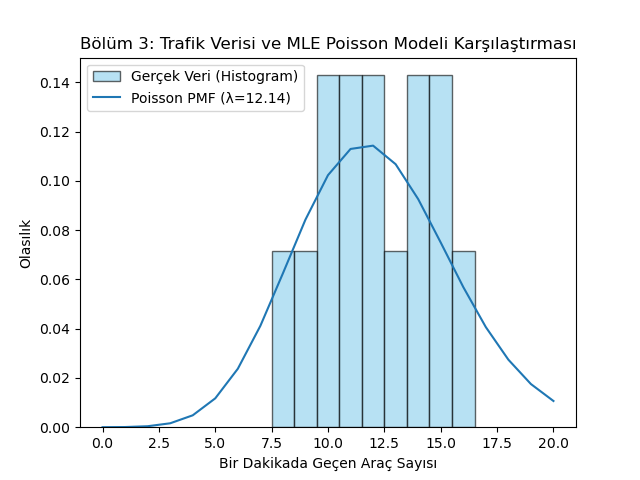
\includegraphics[width=0.8\textwidth]{Figure_1.png}
		\caption{Trafik Verisi Histogramı ve Poisson PMF Eğrisi}
	\end{figure}
	
	Her ne kadar histogram tahmin edilen eğrinin dışındaymış gibi dursa
	da veri arttıkça -verinin doğru olduğu varsayılıyor- bu eğrinin temsil kabiliyeti daha iyi görülecek ve eğriye oturacaktır.
	
	\subsection*{Outlier (Aykırı Değer) Analizi}
	
	Poisson dağılımı outlier'lara karşı zayıftır. Her gelen değer hiçbir karşılaştırma ya da başka bir değerlendirme olmadan genel değere direkt etki eder. Outlier direnci olmadığı için PMF ile yapılacak çıktılar bu yolun gerçekte kullanıldığından daha fazla kullanıldığı zannedilecektir. Eğer 200 araçlık sahte ya da yanlış bir veri girdisi olsaydı belediye bu yola boş yere daha fazla kaynak harcamasına yol açabilir. 
	
	
\end{document}